\documentclass[11pt]{article}
\usepackage{geometry}
\usepackage{url}
\geometry{letterpaper,textwidth=500pt,textheight=720pt,tmargin=30pt,
            footskip=24pt,headsep=18pt,headheight=14pt}
\RequirePackage{amsmath}
\usepackage{amssymb}
\usepackage{textcase}
\usepackage{soul}
\usepackage{indentfirst}

\newcommand{\eps}{\varepsilon}
\newcommand{\kron}{\otimes}
\DeclareMathOperator{\diag}{diag}
\DeclareMathOperator{\trace}{trace}
\DeclareMathOperator{\tvec}{vec}
\DeclareMathOperator{\rank}{rank}
\DeclareMathOperator{\tspan}{span}
\DeclareMathOperator*{\minimize}{minimize}
\DeclareMathOperator*{\maximize}{maximize}
\DeclareMathOperator{\subjectto}{subject\ to}

\newcommand{\mat}[1]{\boldsymbol{#1}}
\renewcommand{\vec}[1]{\boldsymbol{\mathrm{#1}}}
\newcommand{\vecalt}[1]{\boldsymbol{#1}}

\newcommand{\conj}[1]{\overline{#1}}

\newcommand{\normof}[1]{\|#1\|}
\newcommand{\onormof}[2]{\|#1\|_{#2}}

\newcommand{\MIN}[2]{\begin{array}{ll} \displaystyle \minimize_{#1} & {#2} \end{array}}
\newcommand{\MINone}[3]{\begin{array}{ll} \displaystyle \minimize_{#1} & {#2} \\ \subjectto & {#3} \end{array}}
\newcommand{\OPTone}{\MINone}
\newcommand{\MINthree}[5]{\begin{array}{ll} \displaystyle \minimize_{#1} & {#2} \\ \subjectto & {#3} \\ & {#4} \\ & {#5} \end{array}}

\newcommand{\MAX}[2]{\begin{array}{ll} \displaystyle \maximize_{#1} & {#2} \end{array}}
\newcommand{\MAXone}[3]{\begin{array}{ll} \displaystyle \maximize_{#1} & {#2} \\ \subjectto & {#3} \end{array}}


\newcommand{\itr}[2]{#1^{(#2)}}
\newcommand{\itn}[1]{^{(#1)}}

\newcommand{\prob}{\mathbb{P}}
\newcommand{\probof}[1]{\prob\left\{ #1 \right\}}

\newcommand{\pmat}[1]{\begin{pmatrix} #1 \end{pmatrix}}
\newcommand{\bmat}[1]{\begin{bmatrix} #1 \end{bmatrix}}
\newcommand{\spmat}[1]{\left(\begin{smallmatrix} #1 \end{smallmatrix}\right)}
\newcommand{\sbmat}[1]{\left[\begin{smallmatrix} #1 \end{smallmatrix}\right]}

\newcommand{\RR}{\mathbb{R}}
\newcommand{\CC}{\mathbb{C}}

\providecommand{\eye}{\mat{I}}
\providecommand{\mA}{\ensuremath{\mat{A}}}
\providecommand{\mB}{\ensuremath{\mat{B}}}
\providecommand{\mC}{\ensuremath{\mat{C}}}
\providecommand{\mD}{\ensuremath{\mat{D}}}
\providecommand{\mE}{\ensuremath{\mat{E}}}
\providecommand{\mF}{\ensuremath{\mat{F}}}
\providecommand{\mG}{\ensuremath{\mat{G}}}
\providecommand{\mH}{\ensuremath{\mat{H}}}
\providecommand{\mI}{\ensuremath{\mat{I}}}
\providecommand{\mJ}{\ensuremath{\mat{J}}}
\providecommand{\mK}{\ensuremath{\mat{K}}}
\providecommand{\mL}{\ensuremath{\mat{L}}}
\providecommand{\mM}{\ensuremath{\mat{M}}}
\providecommand{\mN}{\ensuremath{\mat{N}}}
\providecommand{\mO}{\ensuremath{\mat{O}}}
\providecommand{\mP}{\ensuremath{\mat{P}}}
\providecommand{\mQ}{\ensuremath{\mat{Q}}}
\providecommand{\mR}{\ensuremath{\mat{R}}}
\providecommand{\mS}{\ensuremath{\mat{S}}}
\providecommand{\mT}{\ensuremath{\mat{T}}}
\providecommand{\mU}{\ensuremath{\mat{U}}}
\providecommand{\mV}{\ensuremath{\mat{V}}}
\providecommand{\mW}{\ensuremath{\mat{W}}}
\providecommand{\mX}{\ensuremath{\mat{X}}}
\providecommand{\mY}{\ensuremath{\mat{Y}}}
\providecommand{\mZ}{\ensuremath{\mat{Z}}}
\providecommand{\mLambda}{\ensuremath{\mat{\Lambda}}}
\providecommand{\mSigma}{\ensuremath{\mat{\Sigma}}}
\providecommand{\mTheta}{\ensuremath{\mat{\Theta}}}
\providecommand{\mPbar}{\bar{\mP}}

\providecommand{\ones}{\vec{e}}
\providecommand{\va}{\ensuremath{\vec{a}}}
\providecommand{\vb}{\ensuremath{\vec{b}}}
\providecommand{\vc}{\ensuremath{\vec{c}}}
\providecommand{\vd}{\ensuremath{\vec{d}}}
\providecommand{\ve}{\ensuremath{\vec{e}}}
\providecommand{\vf}{\ensuremath{\vec{f}}}
\providecommand{\vg}{\ensuremath{\vec{g}}}
\providecommand{\vh}{\ensuremath{\vec{h}}}
\providecommand{\vi}{\ensuremath{\vec{i}}}
\providecommand{\vj}{\ensuremath{\vec{j}}}
\providecommand{\vk}{\ensuremath{\vec{k}}}
\providecommand{\vl}{\ensuremath{\vec{l}}}
\providecommand{\vm}{\ensuremath{\vec{l}}}
\providecommand{\vn}{\ensuremath{\vec{n}}}
\providecommand{\vo}{\ensuremath{\vec{o}}}
\providecommand{\vp}{\ensuremath{\vec{p}}}
\providecommand{\vq}{\ensuremath{\vec{q}}}
\providecommand{\vr}{\ensuremath{\vec{r}}}
\providecommand{\vs}{\ensuremath{\vec{s}}}
\providecommand{\vt}{\ensuremath{\vec{t}}}
\providecommand{\vu}{\ensuremath{\vec{u}}}
\providecommand{\vv}{\ensuremath{\vec{v}}}
\providecommand{\vw}{\ensuremath{\vec{w}}}
\providecommand{\vx}{\ensuremath{\vec{x}}}
\providecommand{\vy}{\ensuremath{\vec{y}}}
\providecommand{\vz}{\ensuremath{\vec{z}}}
\providecommand{\vpi}{\ensuremath{\vecalt{\pi}}}

\providecommand{\vlambda}{\ensuremath{\vecalt{\lambda}}}
\providecommand{\vdelta}{\ensuremath{\vecalt{\delta}}}
\providecommand{\vtheta}{\ensuremath{\vecalt{\theta}}}


\sodef\allcapsspacing{\upshape}{0.15em}{0.65em}{0.6em}%

\DeclareMathOperator*{\argmin}{arg\,min}
\DeclareMathOperator*{\argmax}{arg\,max}

\makeatletter
\def\maketitle{%
\par
\hrule height 0.75pt\vspace{1ex}
\par\noindent
\begin{minipage}{0.75\textwidth}
\scshape
purdue university $\cdot$ project draft \\
Contrastive Learning to Distentagle Motion
\end{minipage}
\begin{minipage}{0.25\textwidth}
\raggedleft
\MakeTextUppercase{\allcapsspacing{\@title}}\\[0.2ex]
\textit{\@author}\\[0.2ex]
\textit{\@date}
\end{minipage}
\par\vspace{1ex}
\hrule height 1pt
\vspace{2ex}
\par
}
\usepackage{mathtools}
\usepackage{animate}
\usepackage{xcolor}
\usepackage{mdframed}
\usepackage{verbatim}
\newenvironment{jcode}{\mdframed[backgroundcolor=blue!20,linecolor=black,leftmargin=20,rightmargin=20]\verbatim\underline{Julia Code}}{\endverbatim\endmdframed}
\usepackage[ruled,vlined,linesnumbered,]{algorithm2e}
%\usepackage{algorithmic}
\usepackage{parskip}
\newcommand{\algrule}[1][.2pt]{\par\vskip.5\baselineskip\hrule height #1\par\vskip.5\baselineskip}
\usepackage{hyperref,xcolor}
\usepackage{comment}


\makeatother


\usepackage[numbers]{natbib}

\author{Kent Gauen}
\title{Draft}

\begin{document}

\maketitle

\section{Overview}

The purpose of this project is to disentangle static and dynamic features of an image.
Recent works have show the ability to decouple features and transformations among scenes~\cite{liu2020learning}. Contrastive learning~\cite{chen2020simple,xiao2020should} is a scheme to learn an encoder invariant to a set of user-defined transformations. Further work has demonstrated by modifying the transformation class, the user is able to modify the invariant class of transformations~\cite{xiao2020should}. Based on these ideas, we propose the following project:

Contrastive learning gives us an encoding of the input image $x$, $\tt{enc}_{CL}(x)$. We would like to maintain complete information of the original image, while still providing the encoded representation of the image. In other words, we want to take the original image $x$ and apply a representation function $\tt{repr}(x) = \tt{enc}_{CL}(x) \cup \tt{enc}_{DI}(x)$ where the information contained in encodings are disjoint. Note $\tt{enc}_{DI}(x)$ is the \emph{disentangled information} of image $x$. 

We would like to answer the following questions:


\begin{itemize}
\item How can contrastive learning be used to disentangle simple information, e.g. noise, from an image? Can we test the disentangle encoder to generate specified noise?
\item Similar to related work~\cite{xiao2020should}, can we use disentangled representations to capture dynamic lighting?
\item How can we apply contrastive learning to decouple static and dynamic image features?
%\item With our trained $\tt{enc}_{CL}(x) = \tt{enc}_{\text{static}}(x)$ and $\tt{enc}_{DI}(x) = \tt{enc}_{\text{dynamic}}(x)$ , can we use generate new dynamic features on the static scene?
%\item With our trained $\tt{enc}_{CL}(x) = \tt{enc}_{\text{static}}(x)$ and $\tt{enc}_{DI}(x) = \tt{enc}_{\text{dynamic}}(x)$ , can we use generate the next frame in the sequence?
\end{itemize}


\section{Progress Overview}

Complete

\begin{itemize}
\item Contrastive learning: code
\item Contrastive learning: train on cifar-10
\item Contrastive learning: test on cifar-10
\item Image Reconstruction: code
\end{itemize}

In progress

\begin{itemize}
\item Image Reconstruction: train on cifar-10  (10 of +1000 epochs)
\end{itemize}


To do

\begin{itemize}
\item Image Reconstruction: test on cifar-10
\item Image Reconstruction: train on face dataset
\item Image Reconstruction: test on face dataset
\item Write down the decoupling mechanism for noisy images
\item Disentanglement Network: code
\item Disentanglement Network: train on cifar-10
\item Disentanglement Network: test on cifar-10
\item Identify more related work
\end{itemize}

\section{Disentangling Model Overview}

\begin{figure}[h]
  \centering
  \includegraphics[width=0.65\linewidth]{figs/disent_model}
  \caption{This figure shows the logic of the disentanglement model.}
\end{figure}

\begin{align}
  L_{simCLR} = \sum_{i \neq j} \rho(z_i,z_j)
\end{align}

\begin{align}
  L_{disent} = \sum_{i \neq j} \rho(g_i,\hat{g}_{i,j})
\end{align}


\newpage
\section{Related Model Overview}

\begin{figure}[h]
  \centering
  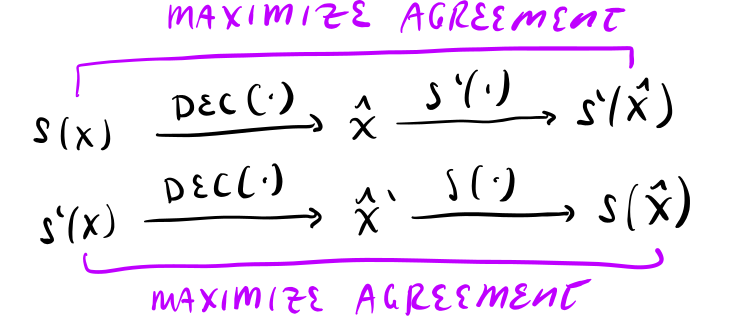
\includegraphics[width=0.65\linewidth]{figs/imgrec_model}
  \caption{This figure shows the logic of the image reconstruction model outlined in~\cite{xia2019training}}
\end{figure}


\begin{figure}[h]
  \centering
  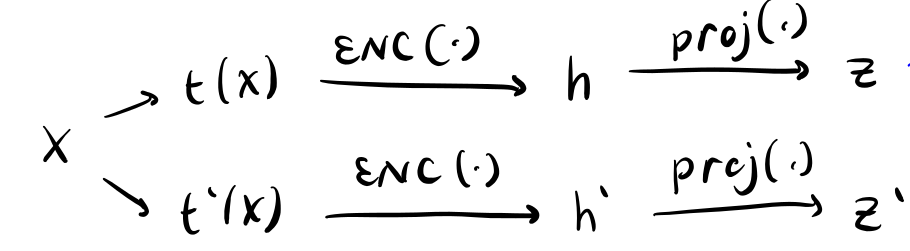
\includegraphics[width=0.65\linewidth]{figs/simclr_model}
  \caption{This figure shows the logic of the simple contrastive learning model outlined in~\cite{chen2020simple}}
\end{figure}

\begin{figure}[h]
  \centering
  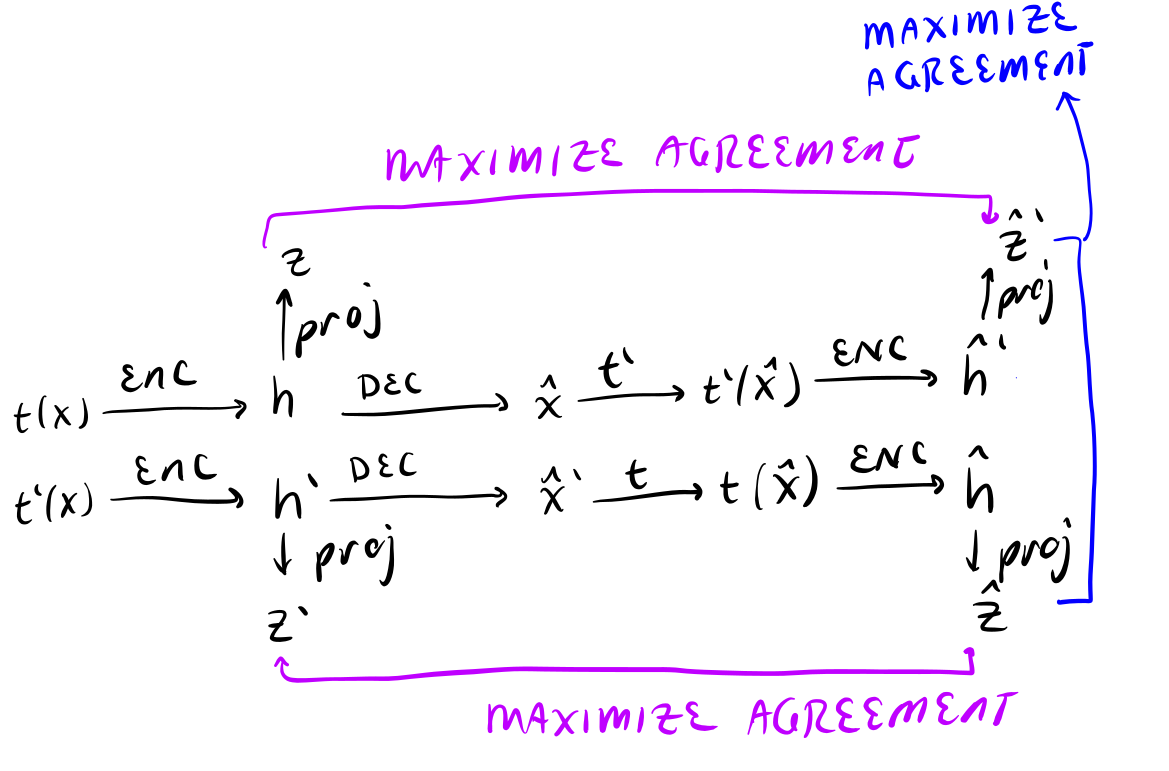
\includegraphics[width=0.75\linewidth]{figs/imgrec_simclr_model}
  \caption{({\tt{new!}}) This figure shows the logic of the combination of simple contrastive learning model and image reconstruction models. This framework removes the need to the training data to provide enough transformation diversity, provided we are able to generate the transformations on our own data set.}
\end{figure}


\newpage
\section*{Related Work}


\newpage

\bibliographystyle{abbrvnat}
\bibliography{ref}


\end{document}


% auto generate a title
% \AtBeginDocument{\maketitle}
